This activity covers user stories US-006 to US-009 and US-041. The component lets a researcher describe a search in natural language, obtain a draft of YouTube Data API parameters from a pre-trained LLM, correct it and save it only when it is valid.

\subsection{Translation: the model proposes, the application decides}

The LLM is not allowed to write YouTube parameters. The request sent to the OpenAI Responses API includes a JSON schema with \texttt{strict} mode enabled \autocite{openai_structured_outputs}, which restricts the answer to the eight typed fields of Table~\ref{tab:llm_draft_fields}. The backend then builds the \texttt{search.\allowbreak list} parameters from those fields: it adds the fixed values \texttt{part=snippet} and \texttt{type=video}, sets \texttt{maxResults}, YouTube's number of results per page, to the number of videos requested but at most 50, the maximum YouTube accepts per page, and leaves out every field the model returned as \texttt{null}. The full number of videos is kept separately as the run's cap, and the collector requests further pages until it is reached (Activity~\ref{act:2.1}). The model therefore cannot invent or misspell a parameter name, and every value it returns is checked again in Python before it is used, because a strict schema guarantees the shape of the answer but not that its values are acceptable to YouTube.

Figure~\ref{fig:translation_example} follows a real request through these steps, from the researcher's prompt to a saved query: the first topic of the validation in Activity~\ref{act:4.3}.

\begin{figure}[htbp]
    \centering
    \begin{tikzpicture}
        [
        node distance=5mm,
        stage/.style={draw, rounded corners=2pt, align=left, font=\footnotesize, text width=9.6cm, inner sep=5pt},
        actor/.style={font=\footnotesize\itshape, align=right, text width=2.4cm},
        flow/.style={-{Stealth[length=2mm]}}
        ]
        \node[stage] (prompt) {\textbf{1. Prompt (researcher)}\\
            \enquote{Videos en español sobre el sistema de transporte masivo MIO de Cali publicados en 2025, ordenados por número de vistas; necesito unos 15 videos.}};
        \node[stage, below=of prompt] (draft) {\textbf{2. Typed draft (LLM, strict JSON schema)}\\
            \texttt{search\_term}: \texttt{MIO Cali transporte masivo}\\
            \texttt{published\_after}: \texttt{2025-01-01T00:00:00Z}\\
            \texttt{published\_before}: \texttt{2026-01-01T00:00:00Z}\\
            \texttt{max\_videos\_to\_discover}: \texttt{15}\\
            \texttt{relevance\_language}: \texttt{es}; \texttt{order}: \texttt{viewCount}\\
            \texttt{region\_code}: \texttt{null}; \texttt{confidence}: \texttt{0.99}};
        \node[stage, below=of draft] (params) {\textbf{3. Parameters built by the backend}\\
            \texttt{part=snippet}, \texttt{type=video}, \texttt{q=MIO Cali transporte masivo}\\
            \texttt{publishedAfter} and \texttt{publishedBefore} as drafted\\
            \texttt{maxResults=15} (page size, at most 50) and a run cap of \texttt{15}\\
            \texttt{relevanceLanguage=es}, \texttt{order=viewCount}\\
            \texttt{regionCode} left out because it is \texttt{null}};
        \node[stage, below=of params] (valid) {\textbf{4. Validation (backend)}\\
            \texttt{validate\_search\_parameters} reports no findings. An invalid value would be reported, never corrected.};
        \node[stage, below=of valid] (review) {\textbf{5. Review and save (researcher)}\\
            \emph{Use these parameters} copies the draft into the form, where the researcher can edit it. On save, the backend validates again and stores the query as \texttt{llm\_generated} with its model, prompt version and confidence.};

        \node[actor, left=4mm of prompt] {browser};
        \node[actor, left=4mm of draft] {OpenAI (LLM)};
        \node[actor, left=4mm of params] {Django backend};
        \node[actor, left=4mm of valid] {Django backend};
        \node[actor, left=4mm of review] {browser and backend};

        \draw[flow] (prompt) -- (draft);
        \draw[flow] (draft) -- (params);
        \draw[flow] (params) -- (valid);
        \draw[flow] (valid) -- (review);
    \end{tikzpicture}
    \caption[Example of the natural-language translation]{Example of the natural-language translation, with the values recorded for the first validation topic on November 10, 2026 (query model \texttt{gpt-6-astra}, prompt version \texttt{v1}). The model only fills the typed fields of step~2; the backend builds the API parameters, caps the page size at 50 while keeping the full number as the run's cap, leaves out empty fields and validates the result before the researcher reviews it.}
    \label{fig:translation_example}
\end{figure}

\begingroup
\setstretch{1.0}
\begin{table}[htbp]
    \centering
    \footnotesize
    \caption{Fields filled by the LLM and the parameters built from them}
    \label{tab:llm_draft_fields}
    \begin{tabularx}
        {\textwidth}{>{\raggedright\arraybackslash}p{4.2cm}>{\raggedright\arraybackslash}p{4.4cm}X}
        \toprule
        \textbf{Draft field}                                  & \textbf{\texttt{search.\allowbreak list} parameter}              & \textbf{Expected format}                  \\
        \midrule
        \texttt{search\_term}                                 & \texttt{q}                                                       & Concise search text                       \\
        \texttt{published\_after}, \texttt{published\_before} & \texttt{publishedAfter}, \texttt{publishedBefore}                & RFC 3339 timestamp in UTC                 \\
        \texttt{max\_videos\_to\_discover}                    & The run's cap, and \texttt{maxResults} as page size (at most 50) & Integer                                   \\
        \texttt{region\_code}                                 & \texttt{regionCode}                                              & ISO 3166 two-letter country code          \\
        \texttt{relevance\_language}                          & \texttt{relevanceLanguage}                                       & ISO 639 two-letter code                   \\
        \texttt{order}                                        & \texttt{order}                                                   & One of the six values accepted by YouTube \\
        \texttt{confidence}                                   & (stored as provenance)                                           & Number between 0 and 1                    \\
        \bottomrule
    \end{tabularx}
\end{table}
\endgroup

The instruction prompt asks for these formats and for \texttt{null} whenever the request does not mention a field, instead of a guess. The prompt has a version identifier that is returned with every draft, together with the model name, so the origin of each draft can be reconstructed. The project's default language is added to the prompt as a hint only when it has the form of a language tag: the interface offers a Spanish/English menu, but the API stores the value as free text, which could otherwise inject instructions into the prompt. Prompts are limited to 2,000 characters.

Failures are reported with distinct HTTP statuses, so the researcher knows what to do next: an empty or too long prompt returns 400, a missing LLM API key returns 503, a refusal by the model returns 422 with its explanation, and a timeout, an upstream error or an unusable answer returns 502 with a generic message. The upstream cause is written to the server log without the API key.

\subsection{Validation of the generated parameters}

A single pure function, \texttt{validate\_\allowbreak search\_\allowbreak parameters}, checks a parameter set against the rules documented for \texttt{search.\allowbreak list}. It reports problems but never corrects them: silently turning \texttt{spanish} into \texttt{es} would change the researcher's request without their knowledge, which a tool for reproducible research must not do. Each finding names the parameter, a stable code (for example \texttt{not\_\allowbreak allowed}, \texttt{missing}, \texttt{invalid\_\allowbreak format} or \texttt{invalid\_\allowbreak range}) and a message for the user.

The rules cover an allowlist of parameter names, the required parameters (\texttt{part}, \texttt{type}, \texttt{q} and \texttt{maxResults}), value types, the exact RFC 3339 layout of dates followed by a calendar check, a start date not later than the end date, the formats of region and language codes, the allowed values of \texttt{order} and an integer \texttt{maxResults} between 0 and 50, in which Boolean values are rejected explicitly because Python treats them as integers. The allowlist also includes ten filters that the researcher sets by hand and the LLM does not fill, such as video duration, captions, license, channel, category and location, each validated against the values documented by YouTube; \texttt{location} and \texttt{locationRadius} must be given together, and the radius cannot exceed 1,000 km.

The same function is applied at three points: when a draft is generated, when a query is saved and when a run starts. The three points can therefore never disagree on what is valid, and an invalid value never reaches YouTube or consumes quota.

Figure~\ref{fig:draft_panel} shows how the interface presents a draft with its validation result, for the same request as Figure~\ref{fig:translation_example}, drafted again live when the screenshot was taken. Its search term, \texttt{sistema de transporte masivo MIO Cali}, differs from the one drafted for the validation run, \texttt{MIO Cali transporte masivo}: the same prompt can produce different drafts, which is why the parameters, not the model's output, are what the researcher reviews and saves.

\begin{figure}[htbp]
    \centering
    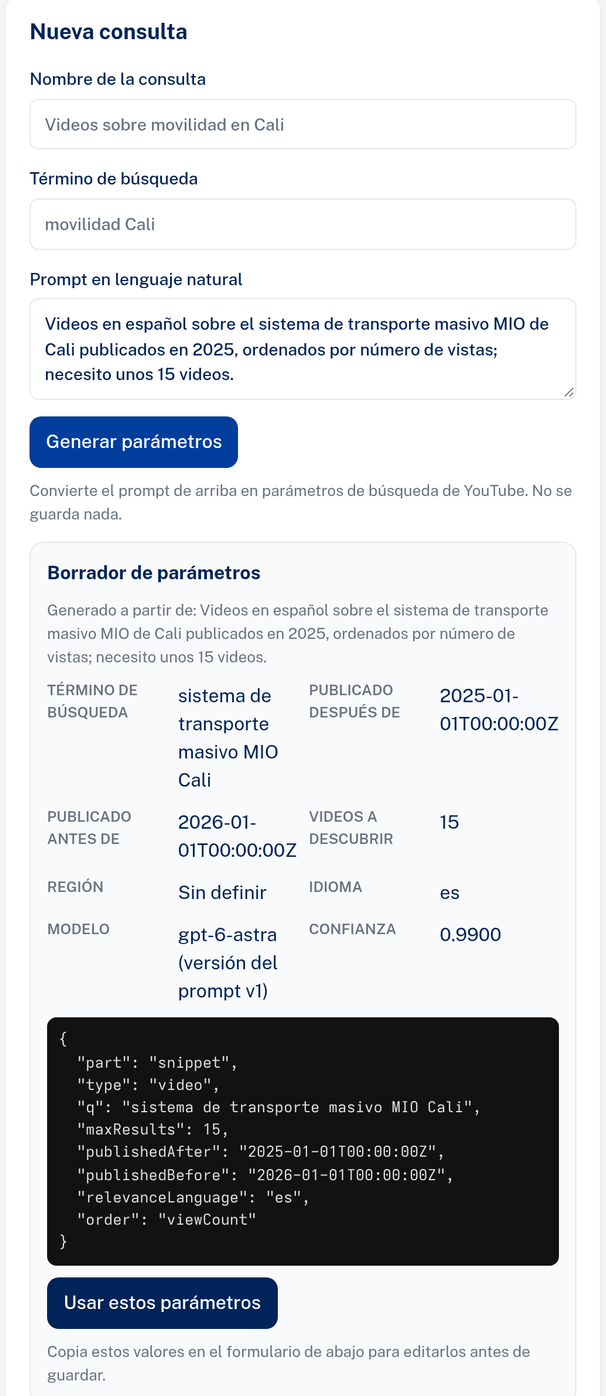
\includegraphics[width=0.55\textwidth]{screenshots/draft-panel-crop.png}
    \caption[The draft panel of the query form]{The draft panel of the query form, cropped: the prompt, the typed draft with its model, prompt version and confidence, and the parameters that \emph{Use these parameters} would copy into the form; no validation finding is listed because the draft passed validation. Real request, November 10, 2026; the interface is in Spanish, its default language.}
    \label{fig:draft_panel}
\end{figure}

\subsection{Review and approval by the researcher}

The draft is shown read-only, with its validation findings, its model, prompt version and confidence. The button \emph{Use these parameters} copies it into the saved-query form, where every value can be edited; the draft remains on screen as the model's original proposal. Dates are converted between the UTC instants expected by YouTube and the local time of the browser's date inputs without losing seconds, so a round trip preserves the same instant.

When the query is saved, the backend validates the parameters again and rejects the save with every finding if any remains, keeping the form unchanged so the researcher can correct it. The provenance of a generated query, formed by the model name, the prompt version and the confidence, is stored only as a complete set and only together with the natural-language prompt it answered; editing the prompt after applying a draft discards it, while editing parameter values keeps it, because reviewing the model's proposal is the purpose of this step. The server, not the browser, sets the query source to \texttt{llm\_\allowbreak generated} or \texttt{manual}. Since the server cannot prove that the browser's provenance was produced by the model, this record documents the origin of a query in a research tool rather than certifying it.
